\documentclass[12pt]{article}

\usepackage{amsmath, amssymb}
\usepackage{bm}
\usepackage{upgreek}
\usepackage{tikz}
\usepackage{tikz-3dplot}
\usepackage{geometry}
\usepackage{float}
\usepackage{comment}
\usepackage{indentfirst}
\usepackage[nottoc]{tocbibind}

% Cross-referencing must be loaded last, and before any \label is used.
% hidelinks suppresses only the coloured border box: the link annotations
% themselves stay, so every \ref, \cite and table-of-contents entry is a
% clickable internal link while the printed page stays black and white.
\usepackage{hyperref}
\hypersetup{
    hidelinks,
    bookmarksnumbered = true,
    pdfstartview = FitH,
    linktoc = all,
}

\setlength{\parindent}{2em}
\geometry{a4paper, margin=1in}

% --- Custom Macros Requested ---
% vectors: boldface, tilde underneath
\newcommand{\vb}[1]{{\underset{\tilde{}}{\mathbf{#1}}}}
% matrices: boldface, underlined
\newcommand{\mb}[1]{\underline{\mathbf{#1}}}
% orthonormal basis {e{}_i}
\newcommand{\bas}[1]{\{ \vb{#1}{}_i \}}
% angular velocity: bold upomega with tilde
\newcommand{\bomega}{\vb{\boldsymbol{\upomega}}}

\title{A rotary self-balancing pendulum visualization through the implementation of LQR control}
\author{Philip Tjuatja}
\date{\today}

\begin{document}
\vspace{15pt}
\maketitle
\newpage
\tableofcontents
\newpage

\section{Introduction and motivation}

This project aims to visualize the behavior of a rotary self-balancing pendulum through the implementation of Linear Quadratic Regulator (LQR) control. The system under consideration is an inverted rotary pendulum, a classic benchmark in nonlinear control theory, first introduced by Furuta, Yamakita and Kobayashi \cite{Furuta1992PseudoState}. The non-linear dynamics of this system make it a challenging yet interesting case study for control engineering, which is a field of interest of mine. I have chosen to implement LQR control for this system due to its optimality properties and its ability to handle multi-variable systems effectively. 

I developed an interest in the topics surrounding this project as after first taking my Intro. to Dynamics and Vibration course (ME2400J) in my university. As a fresh student, visualizing where the math goes and how it translates or connects to real life applications could be tricky at first. Because of this, this project aims to give a clear and intuitive understanding of the system's behavior through visualization of a classical control system. This document will outline the derivation of the equations of motion for the pendulum system, linearization of them around the upright equilibrium point, design of an LQR controller to balance the system, and visualization of the system's response under this control strategy. This is done in hopes that it will give a "goal" for future students stepping into this subject matter, and hence, motivated to learn more about dynamics and its applications in fields like control systems.

\section{Dynamics of the inverted pendulum}

This section aims to derive the model for the pendulum system. I have formulated the question in \S \ref{sec:eom-derivation} that is to be solved in a similar fashion to one that I am familiar with when undergoing my university's Intro. to Dynamics and Vibration course (ME2400J), taught by Prof. Robert G. Parker. The following derivation is done through the methods introduced in the instructor's Essential Dynamics handout~\cite{Parker2026Essential}, specifically from the section for the treatment of Lagrange's equations in Chapter 5: Analytical Dynamics.

\subsection{Derivation of EoM}\label{sec:eom-derivation}
This is a balancing inverted rotary pendulum where a variable moment $M(t)$ is applied about the origin $O$ as shown to keep the pendulum upright. Treatment of these bars are to be rigid bodies; derivations are to neglect dry friction on bearings and viscous drag. Lengths of respective bars are $l{}_A, l{}_B$. Gravity acts in the $-\vb{E}{}_3$ direction. The following are the inertia matrices for both bars about their respective points of reference.
\[
\begin{aligned}
    {}^B\mb{J}^O{}_{\bas{e'}} &= \text{diag}({}^B J{}_1, {}^B J{}_2, {}^B J{}_3) \\
    {}^A\mb{J}^S{}_{\bas{e}} &= \text{diag}({}^A J{}_1, {}^A J{}_2, {}^A J{}_3)
\end{aligned}
\]
Find EoMs for the inverted rotary pendulum.

\begin{figure} [H]
\centering
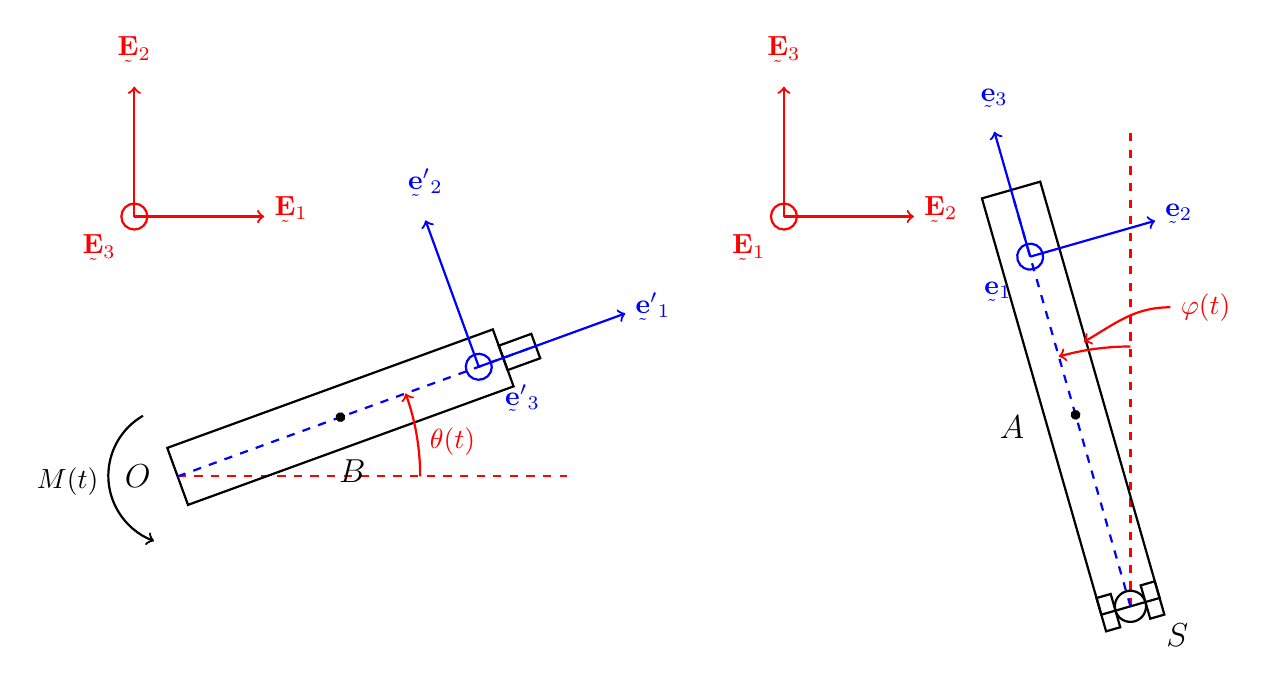
\begin{tikzpicture}[x=1cm, y=1cm, scale=1.1, every node/.style={scale=1}]
    % ==========================================
    % TOP VIEW (Left Side)
    % ==========================================

    % Global Frame E
    \begin{scope}[shift={(-0.5, 3)}]
        \draw[red, thick, ->] (0,0) -- (1.5,0) node[right] {$\vb{E}{}_1$};
        \draw[red, thick, ->] (0,0) -- (0,1.5) node[above] {$\vb{E}{}_2$};
        \draw[red, thick] (0,0) circle (0.15);
        \node[red, anchor=north east] at (-0.1, -0.1) {$\vb{E}{}_3$};
    \end{scope}

    % Arm B & Local Frame
    \begin{scope}[shift={(0,0)}]
        % Base Origin O
        \node[left, font=\large] at (-0.2, 0) {$O$};
        
        % Moment M(t)
        \draw[->, thick] (-0.4, 0.7) arc (120:250:0.8) node[midway, left] {$M(t)$};
        
        % Horizontal Reference Line
        \draw[red, dashed, thick] (0,0) -- (4.5,0);
        
        % Arm B Rotated
        \begin{scope}[rotate=20]
            % Main Arm Rectangle
            \draw[thick] (0, -0.35) rectangle (4, 0.35);
            % End Bracket Rectangle
            \draw[thick] (4, -0.15) rectangle (4.4, 0.15);
            % Centerline
            \draw[blue, dashed, thick] (0,0) -- (4.4,0);
            % Center Dot
            \filldraw[black] (2,0) circle (0.05);
            % Label B
            \node[below, font=\large] at (2, -0.4) {$B$};
            
            % Local Frame e' near the end
            \begin{scope}[shift={(3.7, 0)}] 
                \draw[blue, thick, ->] (0,0) -- (1.8,0) node[right] {$\vb{e}'{}_1$};
                \draw[blue, thick, ->] (0,0) -- (0,1.8) node[above] {$\vb{e}'{}_2$};
                \draw[blue, thick] (0,0) circle (0.15);
                \node[blue, below right] at (0.15, -0.15) {$\vb{e}'{}_3$};
            \end{scope}
        \end{scope}
        
        % Angle theta(t)
        \draw[red, thick, ->] (2.8, 0) arc (0:20:2.8);
        \node[red, right] at (2.8, 0.4) {$\theta(t)$};
    \end{scope}

    % ==========================================
    % FRONT VIEW (Right Side)
    % ==========================================
    \begin{scope}[shift={(7, 0)}]

        % Global Frame E
        \begin{scope}[shift={(0, 3)}]
            \draw[red, thick, ->] (0,0) -- (1.5,0) node[right] {$\vb{E}{}_2$};
            \draw[red, thick, ->] (0,0) -- (0,1.5) node[above] {$\vb{E}{}_3$};
            \draw[red, thick] (0,0) circle (0.15);
            \node[red, anchor=north east] at (-0.1, -0.1) {$\vb{E}{}_1$};
        \end{scope}
        
        % Arm A Pivot Base S
        \coordinate (PivotS) at (4, -1.5);
        
        % Vertical Reference Line
        \draw[red, dashed, thick] (PivotS) -- ++(0, 5.5);
        
        % Arm A Rotated (CCW from vertical)
        \begin{scope}[shift={(PivotS)}, rotate=16] 
            % Side bracket lines (representing the joint)
            \draw[thick] (-0.35, -0.2) rectangle (-0.18, 0.2);
            \draw[thick] (0.18, -0.2) rectangle (0.35, 0.2);
            
            % Main Arm Rectangle A
            \draw[thick] (-0.35, 0) rectangle (0.35, 5);
            % Pivot circle
            \draw[thick] (0,0) circle (0.18);
            % Centerline
            \draw[blue, dashed, thick] (0,0) -- (0, 5);
            % Center Dot
            \filldraw[black] (0, 2.3) circle (0.05);
            % Label A
            \node[left, font=\large] at (-0.5, 2.3) {$A$};
            
            % Label S (red marker at bottom)
            \node[black, right, font=\large] at (0.2, -0.4) {$S$};
            
            % Local Frame e at the top part of the arm
            \begin{scope}[shift={(0, 4.2)}]
                \draw[blue, thick, ->] (0,0) -- (1.5,0) node[right] {$\vb{e}{}_2$};
                \draw[blue, thick, ->] (0,0) -- (0,1.5) node[above] {$\vb{e}{}_3$};
                \draw[blue, thick] (0,0) circle (0.15);
                \node[blue, below left] at (-0.15, -0.15) {$\vb{e}{}_1$};
            \end{scope}
        \end{scope}
        
        % Angle phi(t)
        % Reference vertical is 90 deg, rotated arm is 90 + 16 = 106 deg
        \draw[red, thick, ->] ([shift={(90:3)}]PivotS) arc (90:106:3);
        
        % Pointer and Label for phi(t)
        \draw[red, thick, <-] ([shift={(100:3.1)}]PivotS) to[out=30, in=180] ++(1, 0.4) node[right] {$\varphi(t)$};
        
    \end{scope}
\end{tikzpicture}
\caption{Sketches for the (\textit{left}) top view and (\textit{right}) front view of the rotary inverted pendulum, with bases defined attached.}
\end{figure}

\subsubsection{Define origin and bases}
\label{sec:bases}
We first define the origin $O$ as shown on the figure. The following bases are defined to denote the rotations due to the joints in the arms:
\begin{itemize}
    \item $\bas{E}$ : Fixed basis as shown.
    \item $\bas{e'}$ : Rotate $\bas{E}$ by angle $\theta$ about $\vb{E}{}_3$
    \item $\bas{e}$ : Rotate $\bas{e'}$ by angle $\varphi$ about $\vb{e}'{}_1$
\end{itemize}

Following this, we move away from the usual derivation of the angular velocity matrix and time derivative of bases by means of the rotation matrices and instead utilize the ideas highlighted in Chapter 4.6 of the Essential Dynamics handout \cite{Parker2026Essential}. The angular velocity of the system is given by the addition of the angular velocities of the two rotations, which are expressed in their respective bases. The angular velocity of the system is then expressed in the $\bas{e}$ basis as follows, alongside the time derivatives of the basis vectors $\vb{e}{}_i$:

\begin{center}
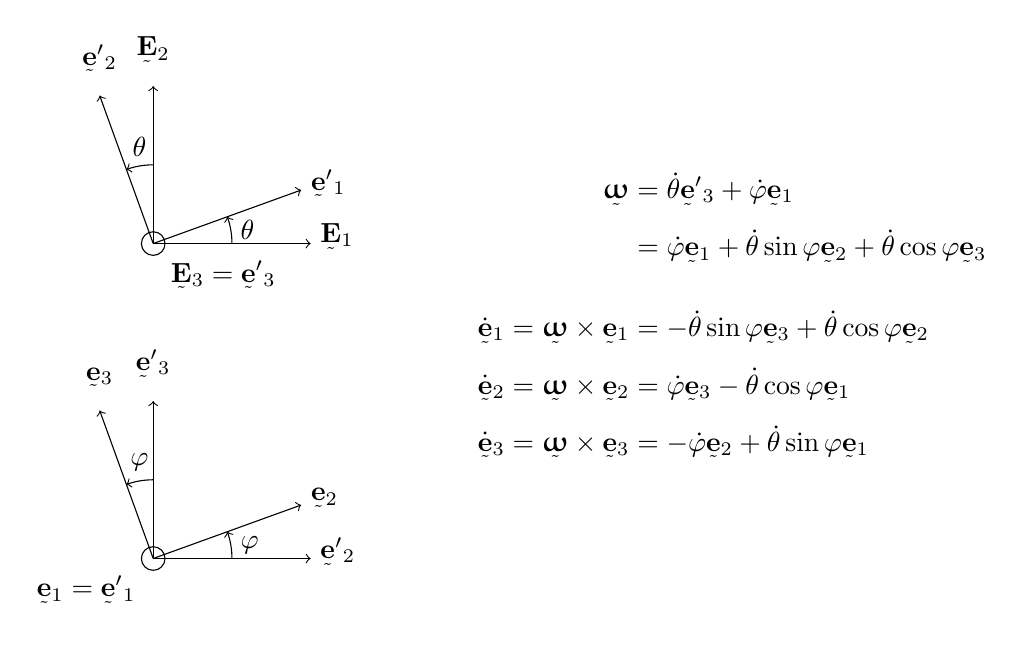
\begin{tikzpicture}[scale=1]
    % Theta rotation
    \draw[->] (0,0) -- (2,0) node[right]{$\vb{E}{}_1$};
    \draw[->] (0,0) -- (0,2) node[above]{$\vb{E}{}_2$};
    \draw[->] (0,0) -- (1.88, 0.68) node[right]{$\vb{e}'{}_1$};
    \draw[->] (0,0) -- (-0.68, 1.88) node[above]{$\vb{e}'{}_2$};
    \draw[->] (1,0) arc (0:20:1) node[midway, right]{$\theta$};
    \draw[->] (0,1) arc (90:110:1) node[midway, above]{$\theta$};
    \draw (0,0) circle (0.15);
    \node[below right] at (0.1,-0.1) {$\vb{E}{}_3 = \vb{e}'{}_3$};

    % Phi rotation
    \begin{scope}[yshift=-4cm]
        \draw[->] (0,0) -- (2,0) node[right]{$\vb{e}'{}_2$};
        \draw[->] (0,0) -- (0,2) node[above]{$\vb{e}'{}_3$};
        \draw[->] (0,0) -- (1.88, 0.68) node[right]{$\vb{e}{}_2$};
        \draw[->] (0,0) -- (-0.68, 1.88) node[above]{$\vb{e}{}_3$};
        \draw[->] (1,0) arc (0:20:1) node[midway, right]{$\varphi$};
        \draw[->] (0,1) arc (90:110:1) node[midway, above]{$\varphi$};
        \draw (0,0) circle (0.15);
        \node[below left] at (-0.1,-0.1) {$\vb{e}{}_1 = \vb{e}'{}_1$};
    \end{scope}
    
    % Math Equations next to it
    \node[anchor=west] at (4, -1) {
        $\begin{aligned}
            \bomega &= \dot{\theta} \vb{e}'{}_3 + \dot{\varphi} \vb{e}{}_1 \\
            &= \dot{\varphi} \vb{e}{}_1 + \dot{\theta} \sin\varphi \vb{e}{}_2 + \dot{\theta} \cos\varphi \vb{e}{}_3 \\[0.3cm]
            \dot{\vb{e}{}}_1 = \bomega \times \vb{e}{}_1 &= -\dot{\theta}\sin\varphi \vb{e}{}_3 + \dot{\theta}\cos\varphi \vb{e}{}_2 \\
            \dot{\vb{e}{}}_2 = \bomega \times \vb{e}{}_2 &= \dot{\varphi}\vb{e}{}_3 - \dot{\theta}\cos\varphi \vb{e}{}_1 \\
            \dot{\vb{e}{}}_3 = \bomega \times \vb{e}{}_3 &= -\dot{\varphi}\vb{e}{}_2 + \dot{\theta}\sin\varphi \vb{e}{}_1
        \end{aligned}$
    };
\end{tikzpicture}
\end{center}

\subsubsection{Kinematics}
Here, we calculate the position, velocity and angular velocities of the centers of mass of both bars. The dot product quantities are calculated to be used in the kinetic energy expression in the next subsection.

 So firstly, for the center of mass of bar B:
\begin{align*}
    \vb{r}{}_B &= \frac{l{}_B}{2} \vb{e}'{}_1 \\
             &= \frac{l{}_B}{2} \vb{e}{}_1 \\
    \dot{\vb{r}}{}_B &= \frac{l{}_B}{2} \dot{\vb{e}}{}_1 \\
             &= \frac{l{}_B}{2} (-\dot{\theta}\sin\varphi \vb{e}{}_3 + \dot{\theta}\cos\varphi \vb{e}{}_2) \\
    \dot{\vb{r}}{}_B \cdot \dot{\vb{r}}{}_B &= \frac{l{}_B^2}{4}\dot{\theta}^2 \\
    \\
    {}^B\bomega &= \dot{\theta} \vb{e}'{}_3 \\
    \\
    {}^B\bomega \cdot {}^B\mb{J} \cdot {}^B\bomega &= {}^B J{}_3 \dot{\theta}^2 
\end{align*}
and using the previous values, for the center of mass of bar A:
\begin{align*}
    \vb{r}{}_A &= \vb{r}{}_B + \frac{l{}_A}{2} \vb{e}{}_3 \\
             &= l{}_B \vb{e}{}_1 + \frac{l{}_A}{2} \vb{e}{}_3 \\
    \dot{\vb{r}}{}_A &= l{}_B (-\dot{\theta}\sin\varphi \vb{e}{}_3 + \dot{\theta}\cos\varphi \vb{e}{}_2) + \frac{l{}_A}{2} (-\dot{\varphi}\vb{e}{}_2 + \dot{\theta}\sin\varphi \vb{e}{}_1) \\
             &= \frac{l{}_A}{2}\dot{\theta}\sin\varphi \vb{e}{}_1 + \left[ -\frac{l{}_A}{2}\dot{\varphi} + l{}_B \dot{\theta}\cos\varphi \right] \vb{e}{}_2 - l{}_B \dot{\theta}\sin\varphi \vb{e}{}_3 \\
    \dot{\vb{r}}{}_A \cdot \dot{\vb{r}}{}_A &= \frac{l{}_A^2}{4}\dot{\theta}^2\sin^2\varphi + \frac{l{}_A^2}{4}\dot{\varphi}^2 + l{}_B^2\dot{\theta}^2\cos^2\varphi + l{}_B^2\dot{\theta}^2\sin^2\varphi - l{}_A l{}_B \dot{\theta}\dot{\varphi}\cos\varphi \\
             &= \frac{l{}_A^2}{4}[\dot{\theta}^2\sin^2\varphi + \dot{\varphi}^2] + l{}_B^2\dot{\theta}^2 - l{}_A l{}_B \dot{\theta}\dot{\varphi}\cos\varphi \\
        {}^A\bomega &= \dot{\varphi} \vb{e}{}_1 + \dot{\theta}\sin\varphi \vb{e}{}_2 + \dot{\theta}\cos\varphi \vb{e}{}_3 \\
        {}^A\bomega \cdot {}^A\mb{J} \cdot {}^A\bomega &= {}^A J{}_1 \dot{\varphi}^2 + {}^A J{}_2 \dot{\theta}^2\sin^2\varphi + {}^A J{}_3 \dot{\theta}^2\cos^2\varphi
\end{align*}


\subsubsection{Forces, Moments and Energy}
Since I chose to use Lagrange's equations to obtain the EoMs, the forces acting on the system are categorized into three groups: conservative, constraint and non-conservative forces/moments.
Conservative forces such that there exist a respective potential:
\begin{itemize}
    \item Gravity: $-m_A g \vb{E}{}_3$ on Bar A and $-m_B g \vb{E}{}_3$ on Bar B. It should be known that there is no contribution from B since there is no change in $\vb{r}{}_B$ in the $\vb{E}{}_3$ direction.
\end{itemize}
There are constraint forces acting on both bars, where identifying them would have been useful for a derivation through balances of linear and angular momentum. However, as these constraints are time-independent, they do not do virtual (and real) work. In this case, we assume for the EoM that there are no non-conservative forces acting on the system. However, there is a non-conservative moment acted on origin $O$, that is, the supplied moment by actuator (due to control system for balancing): \(\vb{M} = M(t)\vb{E}{}_3 \).

So the kinetic and potential energies of the system are given by:
\begin{align*}
    T &= \frac{1}{2}m{}_A \dot{\vb{r}}{}_A \cdot \dot{\vb{r}}{}_A + \frac{1}{2}m{}_B \dot{\vb{r}}{}_B \cdot \dot{\vb{r}}{}_B + \frac{1}{2} {}^A\bomega \cdot {}^A\mb{J} \cdot {}^A\bomega + \frac{1}{2} {}^B\bomega \cdot {}^B\mb{J} \cdot {}^B\bomega \\
      &= \frac{1}{2}m{}_A \left( \frac{l{}_A^2}{4} [\dot{\theta}^2\sin^2\varphi + \dot{\varphi}^2] + l{}_B^2\dot{\theta}^2 - l{}_A l{}_B \dot{\theta}\dot{\varphi}\cos\varphi \right) + \frac{1}{2}m{}_B \frac{l{}_B^2}{4} \dot{\theta}^2 \\
      &\quad + \frac{1}{2}\left( {}^A J{}_1 \dot{\varphi}^2 + \left[ {}^A J{}_2 \sin^2\varphi + {}^A J{}_3 \cos^2\varphi + {}^B J{}_3 \right] \dot{\theta}^2 \right) \\
    V &= m{}_A g \vb{E}{}_3 \cdot \vb{r}{}_A = m{}_A g \, \vb{r}{}_A \cdot (\sin\varphi \vb{e}{}_2 + \cos\varphi \vb{e}{}_3) \\
      &= m{}_A g \frac{l{}_A}{2} \cos\varphi
\end{align*}

\subsubsection{Equations of Motion}
Using classical Lagrange's equations:
\[ \frac{d}{dt} \frac{\partial T}{\partial \dot{q}} - \frac{\partial T}{\partial q} + \frac{\partial V}{\partial q} = \sum \left( \vb{F}^{nc} \cdot \frac{\partial \vb{r}}{\partial q} + \mb{M}^{nc} \cdot \frac{\partial \bomega}{\partial \dot{q}} \right) \]

 Applying to $\theta$: 
\begin{align*}
    \frac{\partial T}{\partial \dot{\theta}} &= \frac{1}{2}m{}_A \left( \frac{l{}_A^2}{4} 2\dot{\theta}\sin^2\varphi + l{}_B^2 2\dot{\theta} - l{}_A l{}_B \dot{\varphi}\cos\varphi \right) + \frac{1}{2}m{}_B \frac{l{}_B^2}{4} 2\dot{\theta} \\ & \quad + \left({}^A J{}_2 \sin^2\varphi + {}^A J{}_3 \cos^2\varphi + {}^B J{}_3\right) \dot{\theta} \\
    \frac{d}{dt}\frac{\partial T}{\partial \dot{\theta}} &= \frac{l{}_A^2}{4} m{}_A \ddot{\theta}\sin^2\varphi + \frac{l{}_A^2}{4} m{}_A \dot{\theta}\dot{\varphi} 2\sin\varphi\cos\varphi + l{}_B^2 m{}_A \ddot{\theta} + m{}_B \frac{l{}_B^2}{4} \ddot{\theta} \\
    &\quad - \frac{l{}_A l{}_B}{2} m{}_A [\ddot{\varphi}\cos\varphi - \dot{\varphi}^2\sin\varphi] + \left({}^A J{}_2 \sin^2\varphi + {}^A J{}_3 \cos^2\varphi + {}^B J{}_3\right) \ddot{\theta} \\
    &= \left[ m{}_A \left( \frac{l{}_A^2}{4}\sin^2\varphi + l{}_B^2 \right) + m{}_B \frac{l{}_B^2}{4} \right] \ddot{\theta} + \left[ \frac{l{}_A^2}{2} m{}_A \sin\varphi\cos\varphi \right] \dot{\theta}\dot{\varphi}\\ &\quad + \left[ {}^A J{}_2 \sin^2\varphi + {}^A J{}_3 \cos^2\varphi + {}^B J{}_3 \right] \ddot{\theta} \\
    &\quad - m{}_A \left[ \left(\frac{l{}_A l{}_B}{2}\cos\varphi\right)\ddot{\varphi} - \left(\frac{l{}_A l{}_B}{2}\sin\varphi\right)\dot{\varphi}^2 \right] \\
    \frac{\partial T}{\partial \theta} &= 0 \quad ; \quad \frac{\partial V}{\partial \theta} = 0 \quad ; \quad (M\sin\varphi \vb{e}{}_2 + M\cos\varphi \vb{e}{}_3) \cdot (\sin\varphi \vb{e}{}_2 + \cos\varphi \vb{e}{}_3) = M \\
    \\
    &\Rightarrow \left[ m{}_A \left(\frac{l{}_A^2}{4}\sin^2\varphi + l{}_B^2\right) + m{}_B \frac{l{}_B^2}{4} \right] \ddot{\theta} + \left[ \frac{l{}_A^2}{2} m{}_A \sin\varphi \cos\varphi \right] \dot{\theta}\dot{\varphi}\\ &\quad + \left[ {}^A J{}_2 \sin^2\varphi + {}^A J{}_3 \cos^2\varphi + {}^B J{}_3 \right]\ddot{\theta} \\
    &\quad - m{}_A \left[ \left(\frac{l{}_A l{}_B}{2}\cos\varphi\right)\ddot{\varphi} - \left(\frac{l{}_A l{}_B}{2}\sin\varphi\right)\dot{\varphi}^2 \right] = M(t)
\end{align*}

 and also for $\varphi$: 
\begin{align*}
    \frac{\partial T}{\partial \dot{\varphi}} &= m{}_A \frac{l{}_A^2}{4} \dot{\varphi} + {}^A J{}_1 \dot{\varphi} - m{}_A \frac{l{}_A l{}_B}{2} \dot{\theta} \cos\varphi\\
    \frac{d}{dt}\frac{\partial T}{\partial \dot{\varphi}} &= \left[ m{}_A \frac{l{}_A^2}{4} + {}^A J{}_1 \right] \ddot{\varphi} - \left[ \left( m{}_A \frac{l{}_A l{}_B}{2} \ddot{\theta} \cos\varphi \right) - \left( m{}_A \frac{l{}_A l{}_B}{2} \dot{\theta}\dot{\varphi} \sin\varphi \right) \right] \\
    \frac{\partial T}{\partial \varphi} &= \frac{1}{2} m{}_A \frac{l{}_A^2}{4} \dot{\theta}^2 \cdot 2\sin\varphi\cos\varphi + m{}_A \frac{l{}_A l{}_B}{2} \dot{\theta}\dot{\varphi}\sin\varphi \\
    &\quad + {}^A J{}_2 \dot{\theta}^2 \sin\varphi\cos\varphi - {}^A J{}_3 \dot{\theta}^2 \cos\varphi\sin\varphi \\
    \frac{\partial V}{\partial \varphi} &= -m{}_A g \frac{l{}_A}{2} \sin\varphi \quad; \quad(M\sin\varphi \vb{e}{}_2 + M\cos\varphi \vb{e}{}_3) \cdot (\vb{e}{}_1) = 0\\
    \\
    &\Rightarrow \left[ m{}_A \frac{l{}_A^2}{4} + {}^A J{}_1 \right] \ddot{\varphi} - \left[ m{}_A \frac{l{}_A^2}{4} + {}^A J{}_2 - {}^A J{}_3 \right] \dot{\theta}^2\sin\varphi\cos\varphi \\ &\quad - \left( m{}_A \frac{l{}_A l{}_B}{2} \right) \ddot{\theta} \cos\varphi - m{}_A g \frac{l{}_A}{2} \sin\varphi = 0
\end{align*}

 Hence, the following equations are the model for the rotary inverted pendulum system:
\begin{equation}
    \begin{aligned}
    &\left[ m{}_A \left(\frac{l{}_A^2}{4}\sin^2\varphi + l{}_B^2\right) + m{}_B \frac{l{}_B^2}{4} \right] \ddot{\theta} + \left[ \frac{l{}_A^2}{2} m{}_A \sin\varphi\cos\varphi \right] \dot{\theta}\dot{\varphi} \\
    &\quad + \left[ {}^A J{}_2 \sin^2\varphi + {}^A J{}_3 \cos^2\varphi + {}^B J{}_3 \right]\ddot{\theta} \\
    &\quad - m{}_A \left[ \left(\frac{l{}_A l{}_B}{2}\cos\varphi\right)\ddot{\varphi} - \left(\frac{l{}_A l{}_B}{2}\sin\varphi\right)\dot{\varphi}^2 \right] & &= M(t) \\
    \\
    &\left[ m{}_A \frac{l{}_A^2}{4} + {}^A J{}_1 \right] \ddot{\varphi} - \left[ m{}_A \frac{l{}_A^2}{4} + {}^A J{}_2 - {}^A J{}_3 \right] \dot{\theta}^2\sin\varphi\cos\varphi \\ &\quad - \left(m{}_A \frac{l{}_A l{}_B}{2}\right)\ddot{\theta}\cos\varphi & &=  m{}_A g \frac{l{}_A}{2} \sin\varphi
\end{aligned} 
\label{eq:eom}
\end{equation}
The model is complete since there are 2 unknowns $\theta, \varphi$ and 2 equations in the model. 
\subsection{State-space model}
\label{sec:state-space}

Rewriting (\ref{eq:eom}) in matrix form yields the equation 
$$ \mb{M} \ddot{\vb{q}} + \mb{C} \dot{\vb{q}} = \vb{\boldsymbol{\uptau}}$$
where, by denoting the following terms for simplicity: 
\begin{align*}
    J{}_\theta &= m{}_A l{}_B^2 + m{}_B \frac{l{}_B^2}{4} + {}^B J{}_3 + {}^A J{}_3 , & J{}_\varphi &= m{}_A \frac{l{}_A^2}{4} + {}^A J{}_1, \\
    B &= m{}_A \frac{l{}_A^2}{4} + {}^A J{}_2 - {}^A J{}_3, & L &= \frac{l{}_A l{}_B}{2} m{}_A,
\end{align*}
we obtain the mass matrix $\mb{M}(\vb{q})$, Christoffel matrix $\mb{C}(\vb{q}, \dot{\vb{q}})$ and moment vector $\vb{\boldsymbol{\uptau}}(\vb{q}, t)$ of the system, given in terms of the modal coordinate $\vb{q}$:

$$\mb{M}, \mb{C} \in \mathcal{M}{}_2(\mathbb{R}), \quad \vb{q} = \begin{bmatrix} \varphi \\ \theta \end{bmatrix} ; \quad \vb{\boldsymbol{\uptau}} = \begin{bmatrix} M(t) \\  m{}_A g \frac{l{}_A}{2} \sin\varphi \end{bmatrix} $$

\begin{align*}
    \mb{M} &= \begin{bmatrix} J{}_\theta + B\sin^2\varphi & -L\cos\varphi \\ -L\cos\varphi & J{}_\varphi \end{bmatrix} \\
    \\
    \mb{C} &= \begin{bmatrix} B \dot{\varphi} \sin\varphi\cos\varphi & B \dot{\theta} \sin\varphi\cos\varphi + L \dot{\varphi} \sin\varphi \\ -B \dot{\theta} \sin\varphi\cos\varphi & 0 \end{bmatrix}
\end{align*}


Linearizing at the upright equilibrium, that is \(\vb{q}{}_0 = \dot{\vb{q}}{}_0=\vb{0}\), the matrices yield

\[
\mb{M}{}_0 \equiv \mb{M}(0)=
\begin{bmatrix}
J_\theta & -L\\
-L & J_\varphi
\end{bmatrix},
\qquad
\mb{C}(0,0)=\mb{0},
\]

and since \(\sin \varphi \approx \varphi\) for small $\varphi$, the linearized torque vector is

\[
\vb{\boldsymbol{\uptau}} \approx \begin{bmatrix} M(t) \\  m{}_A g \frac{l{}_A}{2} \end{bmatrix}.
\]
Since $\mb{C}$ is quadratic in its terms, it vanishes in the first-order approximation. So, the equilibrium state yields
\[
\begin{bmatrix}
J_\theta & -L\\
-L & J_\varphi
\end{bmatrix}
\begin{bmatrix}
\ddot\theta\\[2pt]
\ddot\varphi
\end{bmatrix}
=
\begin{bmatrix}
M(t)\\[4pt]
\dfrac{m_A g l_A}{2}\,\varphi
\end{bmatrix}
\]
For $\det \mb{M}_0 = \Delta = J_\theta J_\varphi - L^2 \neq 0$, $\mb{M}_0$ is invertible and thus obtaining the equation
\[
\begin{bmatrix}
\ddot\theta\\[2pt]
\ddot\varphi
\end{bmatrix}
=
\frac{1}{\Delta}
\begin{bmatrix}
J_\varphi & L\\
L & J_\theta
\end{bmatrix}
\begin{bmatrix}
M(t)\\[4pt]
\dfrac{m_A g l_A}{2}\,\varphi
\end{bmatrix}.
\]
which after multiplying, yields the scalar equations
\begin{align*}
    \ddot\varphi &= \frac{L}{\Delta}M(t) + \frac{J_\theta m_A g l_A}{2\Delta}\,\varphi \\
    \ddot\theta &= \frac{J_\varphi}{\Delta}M(t) + \frac{m_A g l_A L}{2\Delta}\,\varphi 
\end{align*}

Using these equations and defining the state vector $\vb{x}=[\varphi \quad \theta \quad \dot{\varphi} \quad \dot{\theta}]^T$, the matrix equation of the model could be linearized to yield a linear state-space model in the form of $\dot{\vb{x}}=\mb{A}\vb{x}+\mb{B}M(t)$, where explicitly is

\begin{equation}
\dot{\vb{x}} =
\begin{bmatrix}
0 & 0 & 1 & 0\\
0 & 0 & 0 & 1\\
\dfrac{m_A g l_A}{2\Delta}J_\theta & 0 & 0 & 0\\[6pt]
\dfrac{m_A g l_A }{2\Delta}L & 0 & 0 & 0
\end{bmatrix}
\vb{x}
+
\begin{bmatrix}
0\\
0\\
\dfrac{L}{\Delta}\\[4pt]
\dfrac{J_\varphi}{\Delta}
\end{bmatrix}
M(t).
\label{eq:linear-state}
\end{equation}


\newpage

\section{Control theory}
\label{sec:control}

Following previously done works on the Furuta pendulum \cite{Furuta1992PseudoState,FantoniLozano2002}, I aim to apply the Linear Quadratic Regression (LQR) from optimal control theory \cite{Kalman1960Contributions,AndersonMoore1990} to balance the pendulum.

\subsection{Consideration on the use of LQR instead of PID control}
\label{sec:lqr-vs-pid}

In the case of the Furuta pendulum, the use of traditional PID control which treats each degree of freedom independently is problematic since \textit{(i)} the system is strongly coupled, as shown by (\ref{eq:eom}); \textit{(ii)} the upright equilibrium is unstable. LQR control solves this problem by treating the coupled states as a multi-variable state simultaneously and optimizing a quantitative cost function for the selected priorities needed for the system.

\subsection{Derivation of LQR theory}
\label{sec:lqr-derivation}
\subsubsection{Infinite horizon continuous-time case}
\label{sec:lqr-continuous}

Consider the infinite horizon quadratic cost functional \(J: \mathcal{X} \times \mathcal{U} \to \mathbb{R}\) defined by

\[
J [\vb{x}(\cdot), \vb{u}(\cdot)] =\int ^\infty _0 \left( \vb{x}{}^T \mb{Q}\vb{x} + \vb{u}{}^T \mb{R} \vb{u}{}\right) dt
\]
where $\vb{x}{}$ satisfies the linear dynamics \(\dot{\vb{x}} = \mb{A}\vb{x} +\mb{B}\vb{u}, \vb{x}(0) = \vb{x}{}_0\). Here, $\vb{x}(t) \in \mathbb{R}^n$ is the state trajectory of the system, $\vb{u}(t) \in \mathbb{R}^m$ denotes the control inputs of the system, $\mb{Q}\in \mathcal{M}_n (\mathbb{R)}$ is the weight state cost matrix which penalizes the deviation from intended state and $\mb{R} \in \mathcal{M}_m (\mathbb{R)}$ is the weight control cost matrix which penalizes for the effort used in control. Both $\mb{Q}$ and $\mb{R}$ are symmetric but $\mb{Q}$ is semi-positive definite and $\mb{R}$ is positive definite. We seek to minimize $J[\vb{x}, \vb{u}]$ by finding an optimal control law for the system.

Using Pontryagin's minimum principle \cite{Pontryagin1962}, the control Hamiltonian is

\[
H(\vb{x}{}, \vb{u}{}, \vb{\boldsymbol{\lambda}}{}) = \vb{x}{}^T \mb{Q}\vb{x} + \vb{u}{}^T \mb{R} \vb{u}{} + \vb{\boldsymbol{\lambda}}{}^T (\mb{A}\vb{x} +\mb{B}\vb{u})
\]
where this changes the constrained optimization problem into an unconstrained one by introducing Lagrange multipliers $\vb{\boldsymbol{\lambda}}(t) \in \mathbb{R}^n$, here given the name \textit{costate vector}. It reflects the sensitivity of the optimal cost to the changes in the state. Optimality conditions from the minimum principle are as follows:
\begin{enumerate}
    \item state equation  \[\dot{\vb{x}} = \frac{\partial H}{\partial \vb{\boldsymbol{\lambda}}{}}=\mb{A}\vb{x} +\mb{B}\vb{u}\]
    \item costate equation \[ \dot{\vb{\boldsymbol{\lambda}}} = -\frac{\partial H}{\partial \vb{\boldsymbol{x}}{}}= -2\mb{Q}\vb{x}{}-\mb{A}^T\vb{\boldsymbol{\lambda}}\]
    \item stationarity condition \[\frac{\partial H}{\partial \vb{u}{}} = 2\mb{R}\vb{u} + \vb{\boldsymbol{\lambda}}{}^T\mb{B}=\vb{0}{}\]
    \[
    \implies\vb{u}{} =-\frac{1}{2}\vb{R}{}^{-1}\vb{\boldsymbol{\lambda}}{}^T\mb{B}
    \]
\end{enumerate}

From here, we obtain the two-point boundary value problem (TPBVP) since $\vb{x}(t)$ evolves forward from $\vb{x}{}(t=0)$ while $\vb{\boldsymbol{\lambda}}{}(t)$ evolves backward. To solve this TPBVP, the linear relationship 
\[
\vb{\boldsymbol{\lambda}}{} = 2 \mb{P}\vb{x}{}
\]
was assumed. Differentiating, we get
\[
\dot{\vb{\boldsymbol{\lambda}}{}} =  2 \dot{\mb{P}}\vb{x}{} +  2 \mb{P}\dot{\vb{x}{}}.
\]
Using the state equation and the stationary condition and equating it to the costate equation, we arrive at
\[
-2\mb{Q}\vb{x}{}-\mb{A}^T (2\mb{P}\vb{x}{} )= 2\dot{\mb{P}}\vb{x}{} + 2\mb{P}\left( \mb{A} \vb{x}{} - \mb{B} \mb{R}^{-1} \mb{B}^T   \mb{P}\vb{x}{}  \right).
\]
For $\vb{x}{}_0 \neq \vb{0}{}$, simplifying and rearranging yields the differential Riccati equation:
\[
 -\dot{\mb{P}}= \mb{A}^T \mb{P} +\mb{P} \mb{A} - \mb{P} \mb{B} \mb{R}^{-1} \mb{B}^T   \mb{P}+\mb{Q}
\]
Recalling that we are considering the infinite horizon case $t \to \infty$ since the objective is for the system to reach a steady state, so $\dot{\mb{P}} = \mb{0}$, and the equation simplifies to the algebraic Riccati equation:
\begin{equation}
        \mb{A}^T \mb{P} +\mb{P} \mb{A} - \mb{P} \mb{B} \mb{R}^{-1} \mb{B}^T   \mb{P}+\mb{Q} =\mb{0}
        \label{eq:riccati-continuous-eq}
\end{equation}
Solving for $\mb{P}$, which is unique and positive-definite for a stabilisable, detectable plant and substituting into the stationary condition \cite{AndersonMoore1990,Laub1979}, the optimal control law is
\begin{equation}
    \vb{u}{} = - \underbrace{\mb{R}^{-1}\mb{B}^T\mb{P}} _{\mb{K}}\vb{x}{}
    \label{eq:control-law-continuous}
\end{equation}
where $\mb{K}$ here is known as the \textit{optimal feedback gain}.

\subsubsection{Infinite horizon discrete-time case}
\label{sec:lqr-discrete}

While the continuous-time formulation provides the theoretical foundation, practical implementation on digital hardware requires a discrete-time equivalent. We now extend the derivation by converting the continuous integrals and derivatives into discrete sums and differences. 

Consider the infinite horizon quadratic cost functional \(J: \mathcal{X} \times \mathcal{U} \to \mathbb{R}\) defined by

\[
J [\vb{x}{}_k, \vb{u}{}_k] = \sum_{k=0}^\infty \left( \vb{x}{}_k^T \mb{Q}\vb{x}{}_k + \vb{u}{}_k^T \mb{R} \vb{u}{}_k \right)
\]
where \(\vb{x}{}_k\) satisfies the discrete linear dynamics \(\vb{x}{}_{k+1} = \mb{A}\vb{x}{}_k + \mb{B}\vb{u}{}_k, \vb{x}{}_0 = \vb{x}{}(0)\). Here, \(\vb{x}{}_k \in \mathbb{R}^n\) is the state vector of the system at step \(k\), \(\vb{u}{}_k \in \mathbb{R}^m\) denotes the control inputs also at step $k$, both \(\mb{Q}\in \mathcal{M}_n (\mathbb{R})\) and \(\mb{R} \in \mathcal{M}_m (\mathbb{R})\) are the same quantities defined previously in the continuous case. We seek to minimize \(J[\vb{x}, \vb{u}]\) by finding an optimal control law for the system.

Following similarly to the continuous case, using the discrete-time Pontryagin's Minimum Principle, the control Hamiltonian is

\[
H_k(\vb{x}{}_k, \vb{u}{}_k, \vb{\boldsymbol{\lambda}}{}_{k+1}) = \vb{x}{}_k^T \mb{Q}\vb{x}{}_k + \vb{u}{}_k^T \mb{R} \vb{u}{}_k + \vb{\boldsymbol{\lambda}}{}_{k+1}^T (\mb{A}\vb{x}{}_k + \mb{B}\vb{u}{}_k)
\]
where this changes the constrained optimization problem into an unconstrained one by introducing Lagrange multipliers (costate vectors) \(\vb{\boldsymbol{\lambda}}{}_k \in \mathbb{R}^n\) at step $k$, . Similar optimality conditions from the minimum principle are obtained as follows:
\begin{enumerate}
    \item state equation  \[\vb{x}{}_{k+1} = \frac{\partial H_k}{\partial \vb{\boldsymbol{\lambda}}{}_{k+1}} = \mb{A}\vb{x}{}_k + \mb{B}\vb{u}{}_k\]
    \item costate equation \[ \vb{\boldsymbol{\lambda}}{}_k = \frac{\partial H_k}{\partial \vb{x}{}_k} = 2\mb{Q}\vb{x}{}_k + \mb{A}^T\vb{\boldsymbol{\lambda}}{}_{k+1}\]
    \item stationarity condition \[\frac{\partial H_k}{\partial \vb{u}{}_k} = 2\mb{R}\vb{u}{}_k + \mb{B}^T\vb{\boldsymbol{\lambda}}{}_{k+1} = \vb{0}{}\]
    \[
    \implies \vb{u}{}_k = -\frac{1}{2}\mb{R}^{-1}\mb{B}^T\vb{\boldsymbol{\lambda}}{}_{k+1}
    \]
\end{enumerate}

From here, we obtain the discrete two-point boundary value problem (TPBVP) since \(\vb{x}{}_k\) evolves forward from \(\vb{x}{}_0\) while \(\vb{\boldsymbol{\lambda}}{}_k\) evolves backward. Similarly, to solve this TPBVP, the linear relationship 
\[
\vb{\boldsymbol{\lambda}}{}_k = 2 \mb{P}\vb{x}{}_k
\]
was assumed. Note that this also implies \(\vb{\boldsymbol{\lambda}}{}_{k+1} = 2 \mb{P}\vb{x}{}_{k+1}\). Substituting this into the stationarity condition yields
\[
\vb{u}{}_k = -\mb{R}^{-1}\mb{B}^T\mb{P}\vb{x}{}_{k+1} = -\mb{R}^{-1}\mb{B}^T\mb{P}(\mb{A}\vb{x}{}_k + \mb{B}\vb{u}{}_k).
\]
Solving for \(\vb{u}{}_k\), we obtain the discrete optimal control law:
\[
\vb{u}{}_k = -(\mb{R} + \mb{B}^T\mb{P}\mb{B})^{-1}\mb{B}^T\mb{P}\mb{A}\vb{x}{}_k.
\]
Substituting \(\vb{\boldsymbol{\lambda}}{}_k = 2 \mb{P}\vb{x}{}_k\) and \(\vb{\boldsymbol{\lambda}}{}_{k+1} = 2 \mb{P}\vb{x}{}_{k+1}\) into the costate equation gives
\[
2\mb{P}\vb{x}{}_k = 2\mb{Q}\vb{x}{}_k + \mb{A}^T (2\mb{P}\vb{x}{}_{k+1}).
\]
Substituting the state equation and the expression for \(\vb{u}{}_k\), simplifying, and rearranging yields the discrete algebraic Riccati equation \cite{CainesMayne1970,Molinari1975}:
\begin{equation}
\mb{P} = \mb{Q} + \mb{A}^T \mb{P} \mb{A} - \mb{A}^T \mb{P} \mb{B} (\mb{R} + \mb{B}^T \mb{P} \mb{B})^{-1} \mb{B}^T \mb{P} \mb{A}.
\label{eq:riccati-discrete}
\end{equation}
Recalling that we are considering the infinite horizon case \(k \to \infty\) since the objective is for the system to reach a steady state, \(\mb{P}\) converges to a constant matrix. The optimal feedback control law is then given by
\begin{equation}
    \vb{u}{}_k = -\mb{K}\vb{x}{}_k, \quad \text{where} \quad \mb{K} = (\mb{R} + \mb{B}^T\mb{P}\mb{B})^{-1}\mb{B}^T\mb{P}\mb{A}.
    \label{eq:control-law-discrete}
\end{equation}

Note that the additional term $\mb{B}^T\mb{P}\mb{B}$ as compared to the continuous-time case in (\ref{eq:control-law-continuous}) is to account for the fact that $\vb{u}{}_k$ affects the state $\vb{x}{}_{k+1}$ before the cost is evaluated at the next step.

\subsection{Solving for the optimal control law}
\label{sec:solving}

Having done the derivation for both cases above, it could be seen that both cases end in a matrix equation for $\mb{P}$ for which no closed-form solution exists. Because of this, a fixed-point iteration \cite{Kleinman1968} could be applied to iteratively solive it; direct spectral methods exist \cite{Laub1979} and are used here only as an independent check. This subsection will describe that iteration and the properties of it that the implementation relies on.

\subsubsection{The sampled plant}
\label{sec:sampled-plant}

The design is carried out on the sampled plant rather than on the continuous pair $(\mb{A}, \mb{B})$ of (\ref{eq:linear-state}), because the moment is held constant by the motor driver between controller updates \cite{AstromWittenmark2011}. At control period $\Delta t$ the zero-order-hold equivalent of the linearised model is
\[
\mb{A}{}_d = e^{\mb{A}\Delta t}, \qquad
\mb{B}{}_d = \int_0^{\Delta t} e^{\mb{A}\sigma}\mb{B}\, d\sigma
= \sum_{k=0}^{\infty} \frac{\mb{A}^k \mb{B}\,\Delta t^{k+1}}{(k+1)!},
\]
so the state propagates as $\vb{x}{}_{k+1} = \mb{A}{}_d\vb{x}{}_k + \mb{B}{}_d M_k$ with $M_k = M(t_k)$, and the cost being minimised is the discrete one of \S\ref{sec:lqr-discrete}, with $\mb{Q}$ and $\mb{R}$ read as weights per sample.

The distinction is not cosmetic at the control rate used. Solving the continuous problem of \S\ref{sec:lqr-continuous} with the same weights returns a controller whose bandwidth is not attainable at the control rate, whereas the sampled problem returns a markedly gentler gain; the two agree only in the limit $\Delta t \to 0$, so the control law implemented is the discrete one of \S\ref{sec:lqr-discrete} throughout. The two designs are compared quantitatively in \S\ref{sec:control-rate}.


\subsubsection{The Riccati map and Riccati iteration}
\label{sec:riccati-iteration}

Recall that we only have a single input, $m = 1$ so $\vb{u} = [M(t)]$, and with the state in \S\ref{sec:state-space}, $\vb{x} = [\varphi \quad \theta \quad \dot{\varphi} \quad \dot{\theta}]^T$, I define the control weighting is a scalar function $s (\mb{P})$ and the gain row $\mb{F}(\mb{P})$ is
\[
s(\mb{P}) = \mb{R} + \mb{B}{}_d^T \mb{P} \mb{B}{}_d \in \mathbb{R},
\qquad
\mb{F}(\mb{P}) = s(\mb{P})^{-1} \mb{B}{}_d^T \mb{P} \mb{A}{}_d \in \mathbb{R}^{1 \times 4}.
\]
In terms of $\mb{F}$ the discrete algebraic Riccati equation of \S\ref{sec:lqr-discrete} reads
\[
\mathcal{R}(\mb{P}) = \mb{Q} + \mb{A}{}_d^T \mb{P} \left( \mb{A}{}_d - \mb{B}{}_d \mb{F}(\mb{P}) \right),
\]
which is that equation itself, because
\[
\mb{A}{}_d^T \mb{P} \mb{B}{}_d \mb{F}(\mb{P})
= \mb{A}{}_d^T \mb{P} \mb{B}{}_d \left( \mb{R} + \mb{B}{}_d^T \mb{P} \mb{B}{}_d \right)^{-1} \mb{B}{}_d^T \mb{P} \mb{A}{}_d .
\]
Hence $\mb{P} = \mathcal{R}(\mb{P})$ holds if and only if $\mb{P}$ solves the discrete algebraic Riccati equation, and the optimal gain corresponding to that $\mb{P}$ is $\mb{K} = \mb{F}(\mb{P})$. Then, the problem is can be shown as the fixed point of the coupled recursion
\[
\mb{P}_{k+1} = \mathcal{R}(\mb{P}_k), \qquad \mb{K}_k = \mb{F}(\mb{P}_k), \qquad \mb{P}_0 = \mb{Q},
\]
and the control law applied is $\vb{u}{}_k = -\mb{K}\vb{x}{}_k$ with $\mb{K} = \lim_{k\to\infty} \mb{K}_k$. The initial condition $\mb{P}_0 = \mb{Q}$ is the recursion that a finite-horizon problem with one step to go would produce, so the infinite-horizon solution is reached as the horizon is extended. Each iteration is a single evaluation of $\mathcal{R}$: at $n = 4$, this leads to $O(n^3)$ complexity, and no matrix inverse is needed since $s(\mb{P})$ is scalar for $m = 1$. This iteration is also known as the \textit{Riccati iteration}.

\subsubsection{Convergence and stability of the iteration}
\label{sec:convergence}
The following could be concluded from the properties of the Riccati map $\mathcal{R}$ and the iteration, due to the algebraic properties of the matrices involved:
\begin{enumerate}
    \item (\textit{Monotonicity}) The map $\mathcal{R}$ is monotone with respect to the positive semi-definite order: $\mb{P} \preceq \mb{P}' \Rightarrow \mathcal{R}(\mb{P}) \preceq \mathcal{R}(\mb{P}')$. Starting from $\mb{P}_0 = \mb{Q} \succeq \mb{0}$ the iterates are therefore non-decreasing.
    \item (\textit{Boundedness}) Since $(\mb{A}{}_d, \mb{B}{}_d)$ is controllable, as the controllability matrix of (\ref{eq:linear-state}) has rank 4, and $\mb{Q} \succ \mb{0}$ for the weights used, the sequence is bounded above by the stabilising solution $\mb{P}_+$.
\end{enumerate}
A monotone bounded sequence in the positive semi-definite order converges \cite{CainesMayne1970}, and its limit is the unique stabilising solution of the discrete algebraic Riccati equation \cite{Molinari1975}. 

Stability of the iterative solution could be checked by the nature of the matrix corresponding to the state of the system, obtained from the dynamics of the system and the control law applied.:
\begin{align*}
    \vb{x}{}_{k+1} &= \mb{A}_d\vb{x}{}_k + \mb{B}_d\vb{u}{}_k \\
    &= \mb{A}_d\vb{x}{}_k - \mb{B}_d\mb{K}_k\vb{x}{}_k \\
    &= (\mb{A}_d - \mb{B}_d\mb{K}_k)\vb{x}{}_k
\end{align*}
The system is stable if and only if the real part of all the eigenvalues of the closed loop matrix $\mb{A}_d - \mb{B}_d\mb{K}_k$ are negative, or equivalently, if the spectral radius $\rho(\mb{A}_d - \mb{B}_d\mb{K}_k) < 1$, such that the limit $\mb{K} = \lim_{k\to\infty} \mb{K}_k$ must satisfy this condition, that is the solution of the discrete algebraic Riccati equation must be asympototically stable. The iteration should therefore run to convergence and never truncated for speed, since intermediate iterates may not yet stabilise the plant. A phrase to say that this limit is stable is ``closed-loop poles inside the unit disc." The measurements confirming each of these properties for the default design are reported in \S\ref{sec:solver-verification}.


\subsubsection{Termination}
\label{sec:termination}

Since $\mb{P}$ scales with $\mb{Q}/\mb{R}$, an absolute stopping rule is not meaningful: the magnitude of $\mb{P}$ at the solution varies by orders of magnitude across the range of weights exposed by the implementation. The implemented test is therefore relative,
\[
\|\mb{P}_{k+1} - \mb{P}_k\|_{\max} \;\leq\; \tau \max\left(1, \|\mb{P}_k\|_{\max}\right), \qquad \tau = 10^{-9},
\]
with a cap of $k_{\max} = 8000$ iterations, and the returned gain is $\mb{F}$ evaluated at the final iterate. The $\max(1, \cdot)$ factor keeps the test meaningful when the weights themselves are small.

Because $\mb{F}$ is a smooth function of $\mb{P}$, an accuracy of order $\tau$ in $\mb{P}$ carries over to $\mb{K}$: the converged gain agrees with a direct solution of the discrete algebraic Riccati equation \cite{Laub1979} to the order of the tolerance, and the residual of the Riccati equation at the returned $\mb{P}$ is $\mathcal{O}(\tau)$ relative to $\|\mb{P}\|_{\max}$, as the stopping rule prescribes. The iteration count, however, is not fixed: it tracks $\tau$ and grows as the control period shortens, since the recursion converges more slowly as the closed-loop spectral radius approaches unity. The cap is therefore a guard against a control period short enough that the recursion is still unconverged, not a tuning parameter --- the iteration should be left to converge rather than truncated. The measured counts, the solver agreement and the behaviour of the cap against $\Delta t$ are reported in \S\ref{sec:termination-verification}.


\newpage

\section{Software implementation}
\label{sec:impl}

The controller designed above is realised in the JavaScript engine \texttt{js/physics.js}, together with the application layer in \texttt{js/simulator.js}, which drives the companion interactive simulator. The engine has no dependencies, no matrix library and no build step: every matrix involved here is at most $4 \times 4$, so matrices are stored as arrays of rows and multiplied by explicit triple loops. This section documents what the code computes, in the order in which it computes it, and quotes the numbers it produces for the default hardware of \S\ref{sec:state-space} --- the slider defaults of the simulator, namely $l_A = 0.25$ m, $l_B = 0.20$ m, $m_A = 0.08$ kg, $m_B = 0.12$ kg and $g = 9.81$ m/s$^2$, with the bars treated as uniform slender rods.

\subsection{Software layout}
\label{sec:layout}

\begin{center}
\small
\begin{tabular}{l p{8.2cm}}
\hline
function & responsibility \\
\hline
\texttt{deriveParams} & hardware $\rightarrow J_\theta, J_\varphi, B, L$, with ${}^A J_1 = {}^A J_2 = m_A l_A^2/3$, ${}^B J_3 = m_B l_B^2/3$ and the axial term ${}^A J_3$ set to the negligible regularising value $10^{-6}$ \\
\texttt{accel}, \texttt{accelLagrange} & the nonlinear EoMs (\ref{eq:eom}) in the matrix form $\mb{M}\ddot{\vb{q}} + \mb{C}\dot{\vb{q}} = \vb{\uptau}$ and in the raw Lagrange form, the latter kept for cross-validation \\
\texttt{stepRK4} & one classical Runge--Kutta step of the nonlinear model \\
\texttt{energy}, \texttt{pendEnergy} & $T + V$, and the swing-up energy with datum at the upright \\
\texttt{linStateSpace} & $(\mb{A}, \mb{B})$ of (\ref{eq:linear-state}) \\
\texttt{expm}, \texttt{discretizeZOH} & $(\mb{A}{}_d, \mb{B}{}_d)$ at the control period \\
\texttt{lqrDiscrete}, \texttt{lqrGains} & the Riccati iteration and the complete design pipeline \\
\texttt{controller}, \texttt{swingTorque}, \texttt{bangTorque} & the finite-state controller and the two swing-up laws \\
\texttt{sensor}, \texttt{lowpass} & encoder noise and velocity filtering \\
\hline
\end{tabular}
\end{center}

The dynamic state is carried as a plain object whose keys are \texttt{th}, \texttt{ph}, \texttt{thd} and \texttt{phd}, and every consumer reads its components by name. No permutation between an input ordering and a state ordering can therefore be introduced by accident: the gain row solved in \S\ref{sec:riccati-iteration} is applied component by component in the mathematical ordering $\vb{x} = [\varphi, \theta, \dot{\varphi}, \dot{\theta}]^T$ fixed in \S\ref{sec:state-space}. The file \texttt{js/simulator.js} owns the clock, the finite-state wiring, the sliders, the charts and the telemetry, and \texttt{test/physics.test.js} exercises the engine headlessly under Node.

\subsection{Linearisation}
\label{sec:linearisation}

\texttt{linStateSpace} assembles $(\mb{A},\mb{B})$ of (\ref{eq:linear-state}) directly, without ever forming the nonlinear mass matrix: it computes $\Delta = J_\theta J_\varphi - L^2$, then $k = (m_A g l_A / 2)/\Delta$, places the two unit entries $A_{13} = A_{24} = 1$, the gravity coefficients $(A_{31}, A_{41}) = k\,(J_\theta, L)$ and $\mb{B} = (0, 0, L/\Delta, J_\varphi/\Delta)^T$. The inertia-variation amplitude $B$ does not appear, since it multiplies $\sin^2\varphi$ and vanishes at the upright equilibrium. For the default hardware the derived constants are

\begin{center}
\begin{tabular}{l l r}
\hline
quantity & expression & value \\
\hline
$J_\theta$ & $m_A l_B^2 + m_B l_B^2/4 + {}^B J_3 + {}^A J_3$ & $6.0010 \times 10^{-3}$ \\
$J_\varphi$ & $m_A l_A^2/4 + {}^A J_1$ & $2.9167 \times 10^{-3}$ \\
$B$ & $m_A l_A^2/4 + {}^A J_2 - {}^A J_3$ & $2.9157 \times 10^{-3}$ \\
$L$ & $m_A l_A l_B / 2$ & $2.0000 \times 10^{-3}$ \\
$\Delta$ & $J_\theta J_\varphi - L^2$ & $1.3503 \times 10^{-5}$ \\
\hline
\end{tabular}
\end{center}

 and the resulting linear model is
\[
\mb{A} = \begin{bmatrix} 0 & 0 & 1 & 0 \\ 0 & 0 & 0 & 1 \\ 43.598 & 0 & 0 & 0 \\ 14.530 & 0 & 0 & 0 \end{bmatrix},
\qquad
\mb{B} = \begin{bmatrix} 0 \\ 0 \\ 148.12 \\ 216.00 \end{bmatrix}.
\]

\subsection{Zero-order-hold discretisation}
\label{sec:zoh-discretisation}

\texttt{discretizeZOH} evaluates the two series of \S\ref{sec:sampled-plant} with \texttt{expm} and a term recursion. The matrix exponential is computed by scaling and squaring with a Taylor series \cite{MolerVanLoan2003,Higham2005}: the argument $\mb{A}\Delta t$ is halved until $\|\cdot\|_{\max} \le 0.05$ (three halvings for the default $\mb{A}$ at $\Delta t = 5$ ms, since $\|\mb{A}\Delta t\|_{\max} = 43.598 \times 5\times10^{-3} = 0.218$), the series $\sum_k \mb{A}^k/k!$ is then accumulated up to 39 terms with an early exit once a term falls below $10^{-16}$, and the result is squared back the same number of times. At that scale the series reaches machine precision in about seven terms, so the loop terminates long before its limit. The input series for $\mb{B}{}_d$ --- an integral of the matrix exponential \cite{VanLoan1978} --- is accumulated in the same style from $k=0$ to $k=59$, reusing successively higher powers of $\mb{A}$, with the factorial evaluated in closed form; it also terminates after a few terms. The result at the control period $\Delta t = 5$ ms is
{\small
\[
\mb{A}{}_d = \begin{bmatrix} 1.000545 & 0 & 5.00091\times10^{-3} & 0 \\ 1.8164\times10^{-4} & 1 & 3.0273\times10^{-7} & 5\times10^{-3} \\ 0.218029 & 0 & 1.000545 & 0 \\ 0.0726642 & 0 & 1.8164\times10^{-4} & 1 \end{bmatrix},
\]
\[
\mb{B}{}_d = \begin{bmatrix} 1.85162\times10^{-3} \\ 2.70009\times10^{-3} \\ 0.740715 \\ 1.08006 \end{bmatrix},
\]
}
which satisfies the expected small-period check $\mb{B}{}_d \to \mb{B}\Delta t = (0,\ 0,\ 0.740580,\ 1.080014)^T$ to four significant figures, and $\mb{A}{}_d \to \mb{I} + \mb{A}\Delta t$ likewise.

\subsection{The Riccati iteration in code}
\label{sec:riccati-code}

The solver is a single function, \texttt{lqrDiscrete}, transcribed below with the middle columns of the loop collapsed (the helper calls \texttt{mmul}, \texttt{madd}, \texttt{msub}, \texttt{mtrans} and \texttt{mmaxabs} are the obvious row-major matrix operations; an unused identity is elided). The comments give the corresponding quantity of \S\ref{sec:riccati-iteration}.

{\small
\begin{verbatim}
function lqrDiscrete(Ad, Bd, Q, R, maxIter, tol) {
  maxIter = maxIter || 8000;
  tol = tol || 1e-9;
  let P = Q.map(r => r.slice());          // P_0 = Q (copied)
  const BT = mtrans(Bd);
  for (let it = 0; it < maxIter; it++) {
    const PB = mmul(P, Bd);               // P B_d
    const S = R + mmul(BT, PB)[0][0];     // s(P), scalar (m = 1)
    const AtP = mmul(mtrans(Ad), P);      // A_d' P
    const BtPA = mmul(BT, mmul(P, Ad));   // B_d' P A_d
    const Fv = BtPA[0].map(v => v / S);   // F(P) = K_k
    const BF = mmul(Bd, [Fv]);            // B_d F
    const Pnew = madd(mmul(AtP, msub(Ad, BF)), Q);   // R(P_k)
    const scale = Math.max(1, mmaxabs(P));
    if (mmaxabs(msub(Pnew, P)) < tol * scale) {
      return { K: Fv, P: Pnew, it };      // converged
    }
    P = Pnew;
  }
  // cap reached: recompute K from the last iterate and return it
  const BtPA = mmul(BT, mmul(P, Ad))[0];
  const BtPB = mmul(BT, mmul(P, Bd))[0][0];
  return { K: BtPA.map(v => v / (R + BtPB)), P, it: maxIter };
}
\end{verbatim}
}

 Read against \S\ref{sec:riccati-iteration}, the loop body is the map $\mathcal{R}$ itself: \texttt{PB} is $\mb{P}\mb{B}{}_d$, \texttt{S} is the scalar $s(\mb{P})$, \texttt{BtPA} is $\mb{B}{}_d^T\mb{P}\mb{A}{}_d$, \texttt{Fv} is $\mb{F}(\mb{P})$, \texttt{BF} is $\mb{B}{}_d\mb{F}(\mb{P})$ and \texttt{Pnew} is $\mb{Q} + \mb{A}{}_d^T\mb{P}(\mb{A}{}_d - \mb{B}{}_d\mb{F}(\mb{P}))$. Three consequences of $m = 1$ are visible in the listing: $s(\mb{P})$ is a plain number so no matrix inverse is ever formed, the gain row is a flat array of four numbers, and $\mb{K}$ is built from the same intermediate products as $\mb{P}_{k+1}$, so the iteration returns the gain at no extra cost.

Two choices deserve comment. First, the stopping test is relative with a floor of unity, exactly the rule of \S\ref{sec:termination}, so one value of $\tau$ behaves identically for the default weights and for the light-weight corner of the slider range. Second, if the cap is reached the function recomputes $\mb{F}$ from the last iterate and returns it instead of failing; that fallback is not converged, and as noted in \S\ref{sec:termination} it is reached only for control periods far shorter than the $5$ ms used here.

\subsection{Design pipeline and the two designs}
\label{sec:design-pipeline}

\texttt{lqrGains} is the three-step pipeline:
\vspace{5pt}
\par \texttt{linStateSpace} $\rightarrow$ \texttt{discretizeZOH} $\rightarrow$ \texttt{lqrDiscrete}, 
\vspace{5pt}
\par\noindent it is the only entry point the application uses \texttt{recomputeGains} in \texttt{js/simulator.js} calls it twice --- once per design --- on startup and again on every change of a weight slider or of a hardware slider, redisplaying both gains. For the two designs used:

\begin{center}
\small
\begin{tabular}{l l l c c}
\hline
design & $\mb{Q}$ & $R$ & iterations & closed-loop poles \\
\hline
balance & $\text{diag}(300, 25, 5, 1.5)$ & $0.012$ & 629 & $0.0027$; $0.9633$; $0.9850 \pm 0.0076i$ \\
capture & $\text{diag}(500, 1, 8, 0.1)$ & $0.008$ & 1533 & $0.0018$; $0.9613$; $0.9944 \pm 0.0048i$ \\
\hline
\end{tabular}
\end{center}

 with gains
\[
\begin{aligned}
\mb{K}_{bal} &= [\,21.5636 \quad -2.2748 \quad 3.5956 \quad -1.5111\,], \\
\mb{K}_{cap} &= [\,14.4030 \quad -0.4586 \quad 2.1603 \quad -0.5337\,],
\end{aligned}
\]
both in the ordering of \S\ref{sec:state-space}, and both with every closed-loop pole inside the unit disc. The capture design is deliberately indifferent to the arm angle --- its weight on $\theta$ is 500 times smaller than its weight on $\varphi$ --- because it is used only while the pendulum is being caught and the arm is allowed to run; the balance design then brings $\theta$ back to zero.

\subsubsection{The control rate and the design}
\label{sec:control-rate}

The choice of the sampled problem over the continuous one, argued on physical grounds in \S\ref{sec:sampled-plant}, is worth quantifying, because at the control rate used the two are far apart. Continuing with the balance weights $\mb{Q} = \text{diag}(300, 25, 5, 1.5)$ and $R = 0.012$, solving the continuous problem of \S\ref{sec:lqr-continuous} gives
\[
\mb{K} \approx [\,419.98 \quad -45.64 \quad 70.11 \quad -30.10\,],
\]
a controller whose slowest poles sit at $\approx -3.0 \pm 1.5i$ rad/s, whereas the sampled problem at $\Delta t = 5$ ms returns
\[
\mb{K} \approx [\,21.56 \quad -2.27 \quad 3.60 \quad -1.51\,],
\]
which is markedly gentler, since a bandwidth of that order is not attainable at $200$ Hz. The two agree only in the limit $\Delta t \to 0$: already at $\Delta t = 0.1$ ms the same weights return a gain fifteen times larger in its first entry, close to the continuous value. This is the quantitative statement of the argument of \S\ref{sec:sampled-plant}, and it is why the control law implemented is the discrete one of \S\ref{sec:lqr-discrete} throughout.

\subsection{Control loop implementation and energy-pumping swing up}
\label{sec:control-loop}

The nonlinear model is integrated with RK4 at 1 kHz ($\Delta t = 1$ ms) while the controller runs at 200 Hz ($\Delta t_c = 5$ ms), that is one control update every fifth physics step, so the moment is held constant over each control interval --- the same zero-order hold that \S\ref{sec:sampled-plant} assumed when the design was discretised.

At each update the measured state is formed from the true state by \texttt{sensor}: Gaussian encoder noise, applied as $0.5\,$level on the two angles and $2.5\,$level on the two rates (the interface default is 0.01 rad and the filter is off by default), followed by a first-order low-pass on both rates with $\alpha = 0.2$. The angles are wrapped to $(-\pi, \pi]$, and the torque is
{\small
\begin{verbatim}
const K = (ctrl.Kp && aPhi > ctrl.phiSafe) ? ctrl.Kp : ctrl.K;
M = -(K[0]*phiW + K[1]*thW + K[2]*s.phd + K[3]*s.thd);
const lim = ctrl.Mmax;
if (lim > 0) M = Math.max(-lim, Math.min(lim, M));
\end{verbatim}
}
\noindent so the gain row switches from the balance design to the capture design while $|\varphi| > 0.12$ rad, and the result is saturated at $\pm M_{max} = 0.5$ N$\cdot$m (the slider allows $0.1$--$1.2$ N$\cdot$m). The saturation is the one part of the arrangement outside the LQR problem, which assumes an unbounded input; it is a hard nonlinearity, and it is a bound the balance controller is deliberately tested against.

Outside the capture zone the torque comes from the energy-pumping swing-up law rather than from the gain \cite{AstromFuruta2000,Spong1996Energy}:
\[
E = \frac{1}{2}J_\varphi \dot{\varphi}^2 + m_A g \frac{l_A}{2}\left(\cos\varphi - 1\right),
\qquad
M = M_{max}\operatorname{sgn}\left(-E\,\dot{\varphi}\cos\varphi\right) - k_{arm}\dot{\theta},
\]
that is, saturated torque in whichever direction increases the energy towards $E_{ref} = 0$, plus an arm-damping term with $k_{arm} = 0.03$ that stops $\theta$ from winding up. The proportional alternative $M = -k_E E \operatorname{sgn}(\dot{\varphi}\cos\varphi)$ is also implemented and exposed through the $k_E$ slider, but the saturated form is the default because it reaches the capture zone fastest while remaining inside the torque limit. With the basis convention of \S\ref{sec:bases} one has $\dot{E} \propto \dot{\varphi}\cos\varphi \cdot M$ to leading order, so the leading minus sign is what makes $E \to E_{ref}$: when the pendulum lacks energy the arm accelerates in the direction of the pendulum's swing.

Because LQR is only valid near the upright equilibrium, the two laws are combined by a finite-state machine with hysteresis \cite{FantoniLozano2002}. The swing-up phase ends when $|\varphi| \le 0.30$ rad with $|\dot{\varphi}| \le 2.5$ rad/s and $|\dot{\theta}| \le 3.0$ rad/s; balance is then held until the pendulum is clearly lost at $|\varphi| > 0.55$ rad, which prevents the two phases from chattering while an aggressive catch is in progress. The capture bound and the torque limit are exposed as sliders, alongside $k_{arm}$, $k_E$ and the sensor noise level, and the robustness runs of \S\ref{sec:controller-tests} leave them at their defaults, since a pendulum that enters the capture zone too fast or too far off-vertical is the one failure mode the linear design cannot survive.

\subsection{Verification of the default gains}
\label{sec:controller-tests}

This subsection collects the measurements that check the default designs against the theory of \S\ref{sec:control}. It is organised by what is being checked: the properties of the Riccati iteration used in \S\ref{sec:convergence}, the stopping rule of \S\ref{sec:termination} together with an independent solve of the Riccati equation, and finally the plant and controller behaviour of the assembled simulator.

\subsubsection{Synthesiser properties}
\label{sec:solver-verification}

The three claims of \S\ref{sec:convergence} were tested by running the iteration on the default design.

\begin{itemize}
    \item \textit{Monotonicity.} The symmetric part of $\mb{P}_{k+1} - \mb{P}_k$ remained positive semi-definite to within $4 \times 10^{-12}$ over 700 iterations of the default design.
    \item \textit{The limit stabilises the plant.} The closed-loop matrix $\mb{A}{}_d - \mb{B}{}_d\mb{K}$ has every eigenvalue inside the unit disc; for the default weights they are $0.0027$, $0.9633$ and $0.9850 \pm 0.0076i$, matching the balance row of the table in \S\ref{sec:design-pipeline}. The pendulum mode is nearly deadbeat at the control rate while the arm mode stays slow, which is the expected split for a pendulum-first weighting.
    \item \textit{Only the limit may be used.} Intermediate iterates do not stabilise the plant: for the default design $\rho(\mb{A}{}_d - \mb{B}{}_d\mb{F}_k) \approx 1.018$ over the first $\sim$100 iterations and crosses below unity only near convergence. The iteration is therefore run to convergence and never truncated for speed.
    \item \textit{Rate.} Writing $\rho = \rho(\mb{A}{}_d - \mb{B}{}_d\mb{K})$, the distance to the limit contracts by a factor $\rho^2$ per iteration; measured over iterations 201--600 of the default design the contraction is $0.97048$, against $\rho^2 = 0.98507^2 = 0.97035$. Equivalently, one decade of accuracy costs $\left[-\log_{10}\rho^2\right]^{-1} = 76.5$ iterations.
\end{itemize}

\subsubsection{Termination and agreement with a direct solve}
\label{sec:termination-verification}

The stopping rule of \S\ref{sec:termination} was exercised across its whole range. $\|\mb{P}\|_{\max}$ is $3.870 \times 10^4$ for the default weights but $2.26 \times 10^2$ for $R = 5$ with the lightest weights, so an absolute rule would need retuning per design while the relative rule does not.

The iteration count tracks the tolerance the way the rate of \S\ref{sec:solver-verification} predicts --- 179 iterations at $\tau = 10^{-3}$, 421 at $10^{-6}$, 629 at $10^{-9}$ and 883 at $10^{-12}$, roughly 76 iterations bought by each further decade. For the default weights the recursion terminates after 629 iterations at
\[
\mb{K} = [\,21.5636 \quad -2.2748 \quad 3.5956 \quad -1.5111\,],
\]
and the control applied is $M_k = -\mb{K}\vb{x}{}_k$, saturated at the motor limit; the second design, weighted far more heavily on the pendulum than on the arm, is used at the capture hand-off and needs 1533 iterations, again as listed in \S\ref{sec:design-pipeline}. Across the whole range of weights exposed by the implementation ($q_\varphi \in [10, 3000]$, $q_\theta \in [0, 200]$, $q_{\dot{\varphi}} \in [0, 60]$, $q_{\dot{\theta}} \in [0, 30]$, $R \in [0.002, 5]$) the count stays between 163 and 1533, so the cap is never approached at the control period used.

It is not unlimited comfort: at a tenfold faster control rate ($\Delta t = 1$ ms) the same design needs 2927 iterations, and at $\Delta t = 0.1$ ms the cap is reached while the recursion is still unconverged --- the returned gain then differs from the converged one by $\approx 16$ in max-norm --- which the fixed control period of 5 ms avoids. This is the sense in which $k_{\max}$ is a guard rather than a tuning parameter, as stated in \S\ref{sec:termination}.

The solved gain was finally checked against an independent solution of the discrete algebraic Riccati equation that shares none of the iteration's numerics. The Riccati iteration approaches $\mb{P}$ as a fixed point of the Riccati map; the reference instead forms the symplectic pencil of the problem and extracts the stabilising solution from its stable deflating subspace, which is the ordered Schur method of Laub \cite{Laub1979} and the approach used by the dense solver \texttt{scipy.linalg.solve\_discrete\_are}. The two are compared on identical inputs, $\mb{A}{}_d$ and $\mb{B}{}_d$ being taken from the engine itself, so only the algorithm differs.

For the default design the gains agree to $5.5 \times 10^{-7}$ in max-norm, a relative difference of $2.6 \times 10^{-8}$, and the capture design to $7.7 \times 10^{-7}$. The residual of the Riccati equation at the $\mb{P}$ returned by the iteration is $3.7 \times 10^{-5}$, that is $9.6 \times 10^{-10}$ relative to $\|\mb{P}\|_{\max}$ as the stopping rule prescribes, while the reference solution achieves $5.1 \times 10^{-10}$, hence the residual is within the tolerance defined previously. The closed-loop poles match those listed in \S\ref{sec:solver-verification} and every one lies inside the unit disc. This check is reproducible: \texttt{test/dare-crosscheck.py} runs it, and \texttt{test/physics.test.js} invokes it as test \texttt{[9b]}, skipping gracefully where SciPy is unavailable.

\subsubsection{Plant and controller tests}
\label{sec:plant-tests}

The engine carries its own two formulations of the dynamics where in the file \texttt{test/physics.test.js}, the matrix form and the raw Lagrange form of (\ref{eq:eom}) agree to $10^{-9}$ over 200 random states; with $M = 0$ the RK4 integration conserves the mechanical energy $T + V$ to better than $10^{-4}$ relative over 10 s.

At the controller level the same test file runs the finite-state machine headlessly: balance holds for 10 s from an initial offset of $0.12$ rad without the pendulum ever exceeding $0.15$ rad, a swing-up from hanging captures in under 8 s and then holds for 40 s, six different initial states all swing up and balance without the arm winding up, a sharp kick of $1.5$ rad/s applied at $t = 6$ s is rejected, noisy sensors at $0.01$ rad still capture and hold, and five different hardware variants --- lighter and heavier pendulums, longer and shorter arms --- all swing up and balance with the same gains. The browser end-to-end suite finally drives the same engine through the simulator page, checking that the gains are genuinely recomputed when a weight changes, that the swing-up from hanging is captured, that a kick given while balancing is rejected, and that the system is still balancing after 30 s of simulated time at four times real speed.


\newpage
\section*{Acknowledgements}
\addcontentsline{toc}{section}{Acknowledgements}
I would like to thank my Intro.~to Dynamics and Vibrations lecturer, Prof. Robert G. Parker for his encouragement when I first brought up the idea of analyzing stability of dynamical systems. Deepseek AI was used in the generation of the initial draft of the report and the implementation of the code in Javascript. I have verified the correctness of the content and made necessary modifications to ensure accuracy and clarity.

\newpage
\bibliographystyle{ieeetr}
\bibliography{main}

\end{document}